\documentclass[a4paper,10pt]{jsarticle}

% レイアウト
\setlength{\textwidth}{\fullwidth}
\setlength{\textheight}{39\baselineskip}
\addtolength{\textheight}{\topskip}
\setlength{\voffset}{-0.5in}
\setlength{\headsep}{0.3in}
\pagestyle{myheadings}

% パッケージ
\usepackage[dvipdfmx]{graphicx}
\usepackage{amsmath,amssymb,epsfig}
\usepackage{bm}
\usepackage{ascmac}
\usepackage{pifont}
\usepackage{multirow}
\usepackage{enumerate}
\usepackage{cases}
\usepackage{type1cm}
\usepackage{cancel}
\usepackage{url}
\usepackage[dvipdfmx]{color}
\usepackage{listings,jlisting}
% 大きな中括弧
\usepackage{cases}

% 定義
\DeclareMathOperator*{\argmin}{arg\,min}
\DeclareMathOperator*{\argmax}{arg\,max}
\def\vec#1{\mbox{\boldmath$#1$}}
\def\R{{\Bbb R}}

% カウンタの設定
\setcounter{section}{0}
\setcounter{subsection}{0}
\setcounter{subsubsection}{0}
\setcounter{equation}{0}

% キャプションの図をFigに変更
\renewcommand{\figurename}{Fig.}
\renewcommand{\tablename}{Tab.}

% 式番号を式(章番号.番号)に
% \makeatletter
% \renewcommand{\theequation}{\arabic{section}.\arabic{equation}}
% \@addtoreset{equation}{section}
% \makeatother

% プログラムに色をつける
\usepackage{color}

\definecolor{codegreen}{rgb}{0,0.6,0}
\definecolor{codegray}{rgb}{0.5,0.5,0.5}
\definecolor{codepurple}{rgb}{0.58,0,0.82}
\definecolor{backcolour}{rgb}{0.95,0.95,0.92}

\lstdefinestyle{mystyle}{
    backgroundcolor=\color{backcolour},
    commentstyle=\color{codegreen},
    keywordstyle=\color{magenta},
    numberstyle=\tiny\color{codegray},
    stringstyle=\color{codepurple},
    basicstyle=\footnotesize,
    breakatwhitespace=false,
    breaklines=true,
    captionpos=b,
    keepspaces=true,
    numbers=left,
    numbersep=5pt,
    showspaces=false,
    showstringspaces=false,
    showtabs=false,
    tabsize=2
}

\lstset{style=mystyle}

% % ドキュメントの開始
\begin{document}

\section{実行方法}
\subsection{動作環境}
LinuxのディストリビューションのひとつであるUbuntuで動作を確認している.
Ubuntuで動作させるための必要なアプリケーションは以下の通りである.

\begin{lstlisting}[basicstyle=\ttfamily\footnotesize, language=Bash, frame=single, firstnumber=1, numbers=left, breaklines=true]
sudo apt-get install build-essential
sudo apt-get install cmake
sudo apt-get install gnuplot
\end{lstlisting}

コンパイル時に必要なビルドシステムはbuild-essentialとcmakeが必要であり,可視化のためにgnuplotを用いている.

\subsection{コンパイル方法と実行方法}

\begin{lstlisting}[basicstyle=\ttfamily\footnotesize, language=Bash, frame=single, firstnumber=1, numbers=left, breaklines=true]
mkdir build
cd build
cmake ..
make
./実行ファイル名
\end{lstlisting}

\section{課題内容}
\subsection{課題1}
\subsubsection{(a)}
$X_0$軸周り,$Y_0$軸周り,$Z_0$軸周り,の順番に回転する計算方法は以下の通りであり,処理結果の図形をFig.~\ref{fig:課題1(a)}に示す.

\begin{eqnarray}
\label{eq:a}
  \left[
    \begin{array}{c}
      x_1\\
      y_1\\
      z_1\\
      1\\
    \end{array}
  \right] =
  \left[
    \begin{array}{cccc}
      1 & 0 & 0 & 0 \\
      0 & \cos{45^\circ} & -\sin{45^\circ} & 0\\
      0 & \sin{45^\circ} & \cos{45^\circ} & 0\\
      0 & 0 & 0 & 1\\
    \end{array}
  \right]\left[
    \begin{array}{c}
      x\\
      y\\
      z\\
      1\\
    \end{array}
  \right]
\end{eqnarray}

\begin{eqnarray}
\label{eq:b}
  \left[
    \begin{array}{c}
      x_2\\
      y_2\\
      z_2\\
      1\\
    \end{array}
  \right] =
  \left[
    \begin{array}{cccc}
      \cos{60^\circ} & 0 & \sin{60^\circ} & 0 \\
      0 & 1 & 0 & 0\\
      \sin{60^\circ} & 0 & \cos{60^\circ} & 0\\
      0 & 0 & 0 & 1\\
    \end{array}
  \right]\left[
    \begin{array}{c}
      x_1\\
      y_1\\
      z_1\\
      1\\
    \end{array}
  \right]
\end{eqnarray}

\begin{eqnarray}
\label{eq:c}
  \left[
    \begin{array}{c}
      x_3\\
      y_3\\
      z_3\\
      1\\
    \end{array}
  \right] =
  \left[
    \begin{array}{cccc}
      \cos{150^\circ} & -\sin{150^\circ} & 0 & 0 \\
      \sin{150^\circ} & \cos{150^\circ} & 0 & 0\\
      0 & 0 & 1 & 0\\
      0 & 0 & 0 & 1\\
    \end{array}
  \right]\left[
    \begin{array}{c}
      x_2\\
      y_2\\
      z_2\\
      1\\
    \end{array}
  \right]
\end{eqnarray}

\begin{figure}[tb]
  \begin{center}
    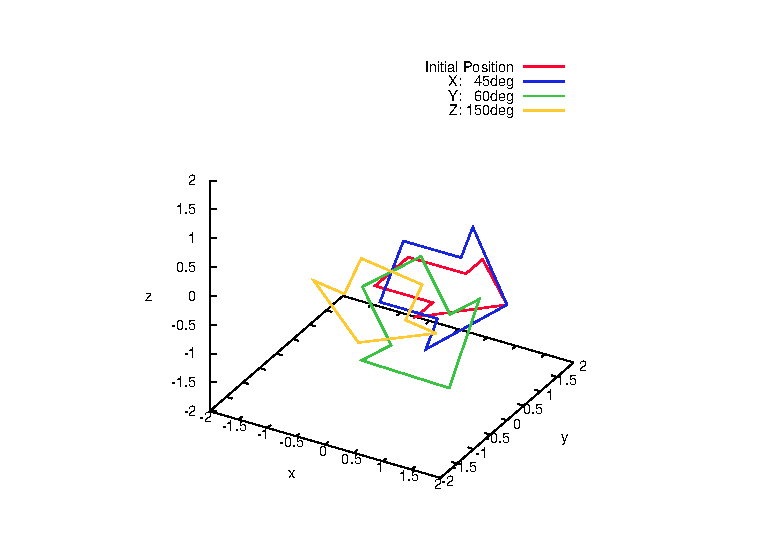
\includegraphics[clip,width=14cm]{fig/eps/1(a).eps}
  \end{center}
  \caption{課題1(a)}
  \label{fig:課題1(a)}
\end{figure}

\subsubsection{(b)}
$Y_0$ 軸周り,$Z_0$軸周り,$X_0$軸周り,の順番に回転する計算方法は以下の通りであり,処理結果の図形をFig.~\ref{fig:課題1(b)}に示す.

\begin{eqnarray}
\label{eq:d}
  \left[
    \begin{array}{c}
      x_1\\
      y_1\\
      z_1\\
      1\\
    \end{array}
  \right] =
  \left[
    \begin{array}{cccc}
      \cos{60^\circ} & 0 & \sin{60^\circ} & 0 \\
      0 & 1 & 0 & 0\\
      \sin{60^\circ} & 0 & \cos{60^\circ} & 0\\
      0 & 0 & 0 & 1\\
    \end{array}
  \right]\left[
    \begin{array}{c}
      x\\
      y\\
      z\\
      1\\
    \end{array}
  \right]
\end{eqnarray}

\begin{eqnarray}
\label{eq:e}
  \left[
    \begin{array}{c}
      x_2\\
      y_2\\
      z_2\\
      1\\
    \end{array}
  \right] =
  \left[
    \begin{array}{cccc}
      \cos{150^\circ} & -\sin{150^\circ} & 0 & 0 \\
      \sin{150^\circ} & \cos{150^\circ} & 0 & 0\\
      0 & 0 & 1 & 0\\
      0 & 0 & 0 & 1\\
    \end{array}
  \right]\left[
    \begin{array}{c}
      x_1\\
      y_1\\
      z_1\\
      1\\
    \end{array}
  \right]
\end{eqnarray}

\begin{eqnarray}
\label{eq:f}
  \left[
    \begin{array}{c}
      x_3\\
      y_3\\
      z_3\\
      1\\
    \end{array}
  \right] =
  \left[
    \begin{array}{cccc}
      1 & 0 & 0 & 0 \\
      0 & \cos{45^\circ} & -\sin{45^\circ} & 0\\
      0 & \sin{45^\circ} & \cos{45^\circ} & 0\\
      0 & 0 & 0 & 1\\
    \end{array}
  \right]\left[
    \begin{array}{c}
      x_2\\
      y_2\\
      z_2\\
      1\\
    \end{array}
  \right]
\end{eqnarray}

\begin{figure}[tb]
  \begin{center}
    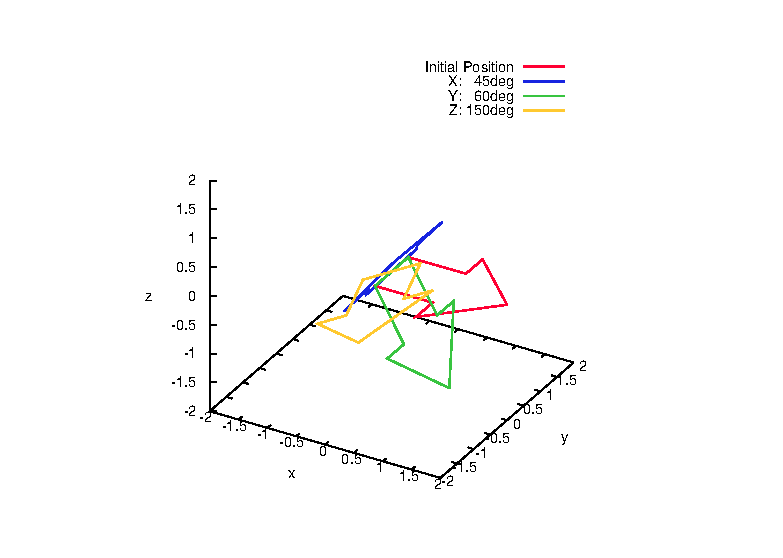
\includegraphics[clip,width=14cm]{fig/eps/1(b).eps}
  \end{center}
  \caption{課題1(b)}
  \label{fig:課題1(b)}
\end{figure}

\subsection{課題2}
任意の原点位置と任意の軸方向を持つ「右手」座標系$O_1X_1Y_1Z_1$を求める.
まず乱数によって任意の原点位置$(x,\ y,\ z)$と$x$軸の方向を決定する単位ベクトルを求めた.
次に$y$軸の方向を決める.
ただし$x$軸と$y$軸は常に直角でなければならないので,$y$軸の方向ベクトルの$x$,$y$成分は乱数で求めた後,内積の関係を用いて$z$成分を決定した.
$z$軸の方向ベクトルは決定した$x$軸と$y$軸の外積を求めることで導出した.
この結果をFig.~\ref{fig:課題1(b)}に示す.

\begin{figure}[htb]
  \begin{center}
    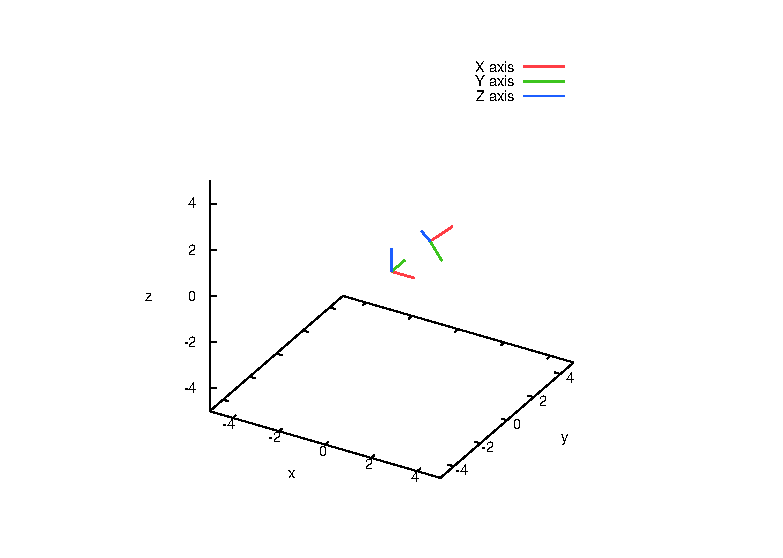
\includegraphics[clip,width=14cm]{fig/eps/2.eps}
  \end{center}
  \caption{課題2}
  \label{fig:課題2}
\end{figure}

\subsection{課題3}

\begin{figure}[htb]
  \begin{center}
    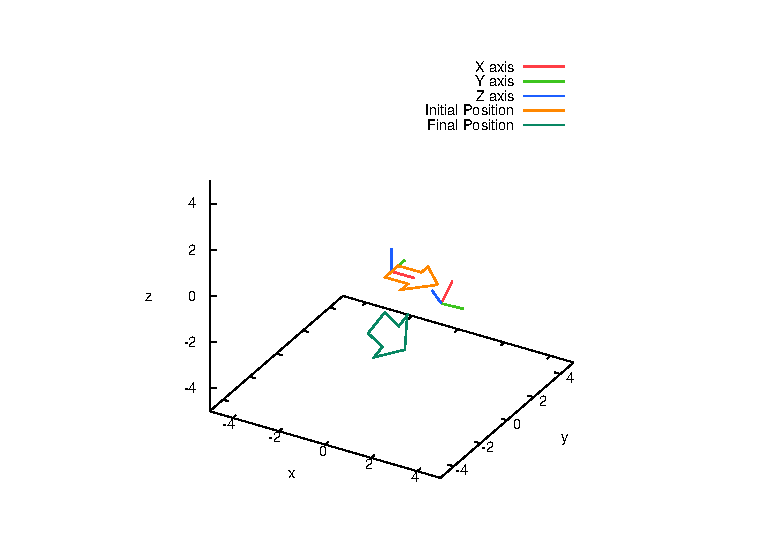
\includegraphics[clip,width=14cm]{fig/eps/3.eps}
  \end{center}
  \caption{課題3}
  \label{fig:課題3}
\end{figure}

\subsection{課題4}
座標系$O_1X_1Y_1Z_1$を基準座標系$O_0X_0Y_0Z_0$に一致させるためには以下の変換行列を定義する.

\begin{eqnarray}
\label{eq:g}
  \left[
    \begin{array}{cccc}
      e_{0x} & e_{1x} & e_{2x} & o_x \\
      e_{0y} & e_{1y} & e_{2y} & o_y\\
      e_{0z} & e_{1y} & e_{2z}& o_z\\
      0 & 0 & 0 & 1\\
    \end{array}
  \right]^{-1}
\end{eqnarray}

式\eqref{eq:g}の$e_{ix}, e_{iy}, e_{iz}$は課題2で求めた座標軸方向ベクトルであり,$o_{x}, y_{y}, z_{z}$は座標系原点の位置ベクトルである.
これを座標系$O_1X_1Y_1Z_1$の座標値と掛けることで,基準座標系$O_0X_0Y_0Z_0$と一致させることができる.

この結果をFig.~\ref{fig:課題4}に示す.Fig.~\ref{fig:課題4}より基準座標系$O_0X_0Y_0Z_0$に一致させた様子は濃緑色の軸で示している.

\begin{figure}[htb]
  \begin{center}
    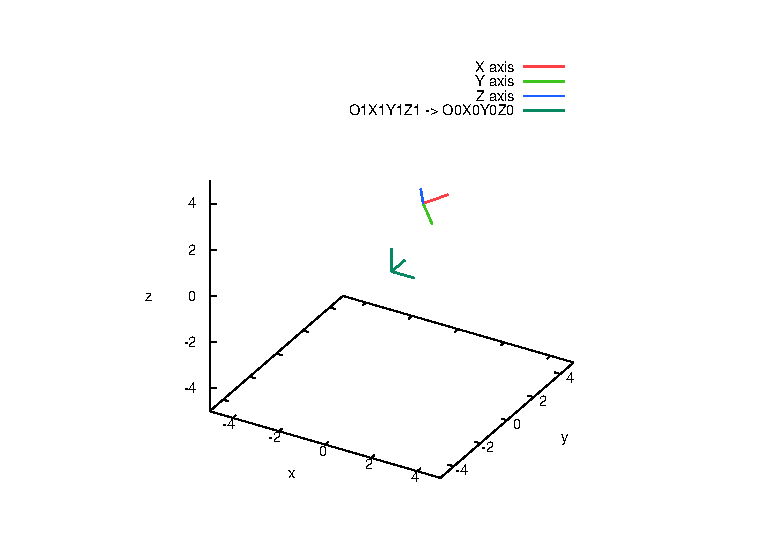
\includegraphics[clip,width=14cm]{fig/eps/4.eps}
  \end{center}
  \caption{課題4}
  \label{fig:課題4}
\end{figure}

\subsection{課題5}
課題3と課題4の解法で導出した矢印を表現する座標値が一致している様子をFig.~\ref{fig:課題5}に示す.
ただし課題3での結果をオレンジ色,課題4で求めた変換によって求めた座標値を濃緑色でそれぞれプロットしているがそれぞれの値が一致しているため,濃緑色の線のみ表示されている.

\begin{figure}[htb]
  \begin{center}
    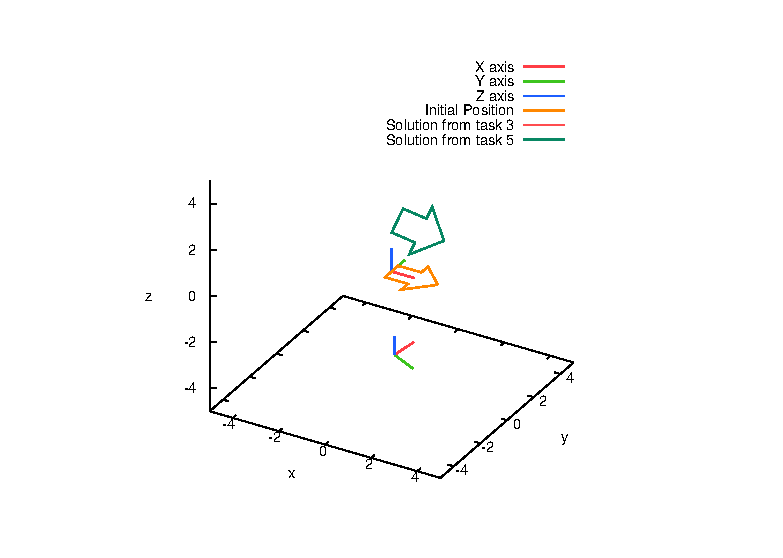
\includegraphics[clip,width=14cm]{fig/eps/5.eps}
  \end{center}
  \caption{課題5}
  \label{fig:課題5}
\end{figure}

\end{document}